
% \textbf{\Large FORMATTING}\vspace{7pt}
\section{FORMATTING}

\subsection{Page Size} 
The page size should be set to A4.

\subsection{Text}
Text must be single-spaced using a Times New Roman font throughout the paper except for main headings which will be Arial Bold. Use an 18-point font for the Title, a 12-point font for Author Name(s), a 12-point font for all Section and Subsection Heads and a 10-point font for all body text.  Text must be full justified.  Do not indent paragraphs; skip one line between paragraphs.

\subsection{Paper Title}
The paper title with Arial, \textbf{bold-faced} in 18-point font should be left justified at the location shown. Maximum of two lines may be used.

\subsection{Author Name(s)}
Author names in Times New Roman 12 point font should consist of first name and middle name initials followed by the complete last name in upper and lower case, left justified under the title in bold.

\subsection{Section and Subsection Heads}

\section{SECTION HEADS} 

\subsection{Subsection Heads} 

\subsubsection{Sub-subsection Heads.}

\textbf{Text Citation of References}

Within text of an article, references are to be cited by last name of author, with “et al,” for multiple authors, and year of publication.   For example:   .....was discovered (Longuet-Higgins et al, 1977)

\hspace{35pt}Ueda and Rashed (1990) proposed …

\hspace{35pt}Sparrow (1980a) discovered ...

\hspace{35pt}It was also noted (Sparrow 1980b; Kheisin 1992) that ...\vspace{7pt}

\textbf{Tables}

Number tables consecutively and use table numbers when referring to a table (for example Table 1, Tables 2 and 3, ...). SI Units must be used for all weights and measures.

\begin{table}[H]
    \centering
    \captionsetup{labelfont={bf}}
    \caption{Table captions should be placed above table, CENTERED}
    \begin{tabular}{|l|c|c|}\hline
         & 1 & 2 \\\hline
         A & & \\\hline
         B & & \\\hline
    \end{tabular}
    \label{tab:my_label}
\end{table}

\textbf{Equations}

Equations are to be numbered consecutively from 1 to the end of the paper right justified in square brackets, Equations in appendices should be renumbered from 1 with the Appendix letter.   For example, Appendix A equations should be A1, A2, etc.  When referring to equations in the text use “Equation 1, equation 2, etc.”. Equations should be in italics and indented. Enclose equation numbers in square brackets and place flush right with right-hand margin of the column, for example Equation \ref{eq:example}.

\begin{equation}
    F(x,y,z;t) = (A_xx^2 + B_yy^3 + Cz)exp(k_xx + \omega t)
    \label{eq:example}
\end{equation}

\textbf{Figures}

Number figures consecutively and use the figure number when referring to a figure (Figure 1) or figures (Figures 2 to 3),... Place Figures/Images in text as close following the reference as possible. Figures must have a caption consisting of the figure number, and brief title and should be placed below figure, centered, as shown below:

\begin{figure}[H]
    \centering
    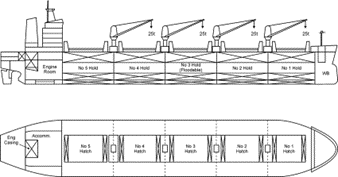
\includegraphics[width=.5\textwidth]{Picture1.png}
    \caption{Example Handymax bulk carrier (Akyar, 2018)}
    \label{fig:enter-label}
\end{figure}

Each appendix should have individual figure numbers.  For example, APPENDIX A figures should be Figure A1, A2, … etc.





